%HW12.tex
%Twelfth Homework -- Math 221H
% 
%
% Frank Sottile
% 11 November 2023 
%
%%%%%%%%%%%%%%%%%%%%%%%%%%%%%%%%%%%%%%%%%%%%%%%%%%%%%%%%
\documentclass[12pt]{article}
\usepackage{amssymb,amsmath}
\usepackage{graphicx}
\usepackage[usenames,dvipsnames,svgnames,table]{xcolor}
\usepackage{multirow}   % This is for more control over tables
%%%%%%%%%%%%%%%%%%%%%%%%%%%%%%%%  Layout     %%%%%%%%%%%%%%%%%%%%%%%%%%%%%%%%%%%%%%
\usepackage{vmargin}
\setpapersize{USletter}
\setmargrb{1cm}{0.25cm}{1cm}{0.5cm} % --- sets all four margins LTRB

%%%%%%%%%%%%%%%%%%%%%%%%%%%%%%%%%%%%%%%%  Macros  %%%%%%%%%%%%%%%%%%%%%%%%%%%%%%%%%%%%%%%%
\newcommand{\RR}{{\mathbb R}}  % This is the backboard bold symbol for the real numbers.  Note how it is used below
\newcommand{\NN}{{\mathbb N}}  % 
\newcommand{\ZZ}{{\mathbb Z}}  %

\newcommand{\calP}{{\mathcal P}}  %Caligraphic P for power set

\newcommand{\bfa}{{\bf a}}    %Vectors
\newcommand{\bfb}{{\bf b}}    %Vectors
\newcommand{\bfF}{{\bf F}}    %Vectors
\newcommand{\bfr}{{\bf r}}    %Vectors
\newcommand{\bfi}{{\bf i}}    %Unit Vectors
\newcommand{\bfj}{{\bf j}}    %Unit Vectors
\newcommand{\bfk}{{\bf k}}    %Unit Vectors

\newcommand{\sep}{{\ :\ }}     % This is for the : in our notation for building sets.
                               % an acceptable (and common) alternative is \mid  (try it!)
%%%%%%%%%%%%%%%%%%%%%%%%%%%%%%%%%%%%%%%%%%%%%%%%%%%%%%%%%%%%%%%%%%%%%%%%
\begin{document}
\LARGE 
\noindent
{\color{Maroon}Honors Multivariate Calculus \hfill Math 221H Section 201}\vspace{2pt}\\
\large
Twelfth Homework:\hfill 
Due in recitation: Thursday 16 November 2023\vspace{2pt}

\normalsize
    \vspace{2pt}

%%%%%%%%%%%%%%%%%%%%%%%%%%%%%%%%%%%%%%%%%%%%%%%%%%%%%%%%%%%%%%%%%%%%%%%%%%%%%%%%%%%%%%%%%%%%%%%%%%%%
\begin{enumerate}



%%%%%%%%%%%%%%%%%%%%%%%%%%%%%%%%%%%%%%%%%%%%%%%%%%%%%%%%%%%%%%%%%%%%%%%%%%%%%%%%%%%%%%%%%%%%%%%%%%%%
\item A 50kg woman carries a 6kg can of paint up a helical staircase the encircles a silo with a radius of 6m and a
  height of 30m.
  How much work does she do against gravity in accomplishing this task?\vspace{-2pt}
%%%%%%%%%%%%%%%%%%%%%%%%%%%%%%%%%%%%%%%%%%%%%%%%%%%%%%%%%%%%%%%%%%%%%%%%%%%%%%%%%%%%%%%%%%%%%%%%%%%%
   
   
%%%%%%%%%%%%%%%%%%%%%%%%%%%%%%%%%%%%%%%%%%%%%%%%%%%%%%%%%%%%%%%%%%%%%%%%%%%%%%%%%%%%%%%%%%%%%%%%%%%%
\item  Suppose now that the paint leaks out of the can at a constant rate (and that she trudges at a constant rate) so that
  1 kg is left when she gets to the top.
  How much work does she do against gravity in accomplishing this task?
  \vspace{-2pt}
%%%%%%%%%%%%%%%%%%%%%%%%%%%%%%%%%%%%%%%%%%%%%%%%%%%%%%%%%%%%%%%%%%%%%%%%%%%%%%%%%%%%%%%%%%%%%%%%%%%%

   
%%%%%%%%%%%%%%%%%%%%%%%%%%%%%%%%%%%%%%%%%%%%%%%%%%%%%%%%%%%%%%%%%%%%%%%%%%%%%%%%%%%%%%%%%%%%%%%%%%%%
\item For each of the following vector fields $\bfF$, determine whether or not it is conservative.
  If it is, find a potential function $f$ such that $\bfF=\nabla f$.\newline 
  (a)\ $\bfF(x,y)=(x^2+y)\bfi + (y^2+x)\bfj$
  \qquad\qquad
  (b)\ $\bfF(x,y)=(\arctan(x)+y)\bfi + (\sin(xy)+x)\bfj$\newline
  (c)\ $\bfF(x,y)=(ye^{xy}+4x^3y)\bfi + (xe^{xy}+x^4)\bfj$
  \vspace{-2pt}
%%%%%%%%%%%%%%%%%%%%%%%%%%%%%%%%%%%%%%%%%%%%%%%%%%%%%%%%%%%%%%%%%%%%%%%%%%%%%%%%%%%%%%%%%%%%%%%%%%%%

%%%%%%%%%%%%%%%%%%%%%%%%%%%%%%%%%%%%%%%%%%%%%%%%%%%%%%%%%%%%%%%%%%%%%%%%%%%%%%%%%%%%%%%%%%%%%%%%%%%%
\item Suppose that $\bfF(x,y,z)$ is a vector function defined on $\RR^{3}\smallsetminus\{(0,0,0)\}$ whose direction at a point  is away
  from the origin and magnitude is proportional to the distance from the origin.

  Show that $\bfF$ is conservative.  \vspace{-2pt}
%%%%%%%%%%%%%%%%%%%%%%%%%%%%%%%%%%%%%%%%%%%%%%%%%%%%%%%%%%%%%%%%%%%%%%%%%%%%%%%%%%%%%%%%%%%%%%%%%%%%

   
%%%%%%%%%%%%%%%%%%%%%%%%%%%%%%%%%%%%%%%%%%%%%%%%%%%%%%%%%%%%%%%%%%%%%%%%%%%%%%%%%%%%%%%%%%%%%%%%%%%%
\item More generally, suppose that $g(t)$ is a continuous function of a nonnegative variable $t$.
  Show that the vector field $\bfF(x,y,z)=g(x^2+y^2+z^2) ( x\bfi + y \bfj + z \bfk)$ is conservative.\vspace{-2pt}
%%%%%%%%%%%%%%%%%%%%%%%%%%%%%%%%%%%%%%%%%%%%%%%%%%%%%%%%%%%%%%%%%%%%%%%%%%%%%%%%%%%%%%%%%%%%%%%%%%%%
   
 
   
%%%%%%%%%%%%%%%%%%%%%%%%%%%%%%%%%%%%%%%%%%%%%%%%%%%%%%%%%%%%%%%%%%%%%%%%%%%%%%%%%%%%%%%%%%%%%%%%%%%%
\item Show that each of the following line integrals are independent of path, and then evaluate the integral, either by finding a propitious
  path or a potential function.
  
  (a)\ ${\displaystyle \int_{(0,0)}^{(1,\pi/2)} e^x \sin y\, dx \ + e^x \cos y\, dy}$
  \qquad
  (b)\ ${\displaystyle \int_{(-1,1)}^{(4,2)} \bigl(y - \frac{1}{x^2}\bigr)\, dx\ +\ \bigl(x - \frac{1}{y^2}\bigr)\, dy}$\vspace{4pt}

  (c)\ ${\displaystyle \int_{(0,0,0)}^{(1,1,1)} (6x y^3 + 2z^2) dx\ +\ 9x^2y^2\,dy\ +\ (4xz+1)dz}$\newline
  (Hint: try a piecewise linear path parallel to coordinate axes.)
 \vspace{-2pt}
%%%%%%%%%%%%%%%%%%%%%%%%%%%%%%%%%%%%%%%%%%%%%%%%%%%%%%%%%%%%%%%%%%%%%%%%%%%%%%%%%%%%%%%%%%%%%%%%%%%%

   
%%%%%%%%%%%%%%%%%%%%%%%%%%%%%%%%%%%%%%%%%%%%%%%%%%%%%%%%%%%%%%%%%%%%%%%%%%%%%%%%%%%%%%%%%%%%%%%%%%%%
\item Show that if the vector field $\bfF= P\bfi + Q\bfj + R\bfk$ is conservative and $P$, $Q$, and $R$ have continuous first-order partial
  derivatives, then\vspace{-4pt}
  \[
  \frac{\partial P}{\partial y}=\frac{\partial Q}{\partial x}\ ,
  \qquad
  \frac{\partial P}{\partial z}=\frac{\partial R}{\partial x}\ , \ \mbox{ and }\ 
  \quad
  \frac{\partial Q}{\partial z}=\frac{\partial R}{\partial y}\ .
  \vspace{-2pt}
  \]
%%%%%%%%%%%%%%%%%%%%%%%%%%%%%%%%%%%%%%%%%%%%%%%%%%%%%%%%%%%%%%%%%%%%%%%%%%%%%%%%%%%%%%%%%%%%%%%%%%%%

%%%%%%%%%%%%%%%%%%%%%%%%%%%%%%%%%%%%%%%%%%%%%%%%%%%%%%%%%%%%%%%%%%%%%%%%%%%%%%%%%%%%%%%%%%%%%%%%%%%%
\item Let ${\displaystyle \bfF(x,y) = \frac{-y\bfi + x \bfj}{x^2+y^2} }$.
  Show that $\partial P/\partial y=\partial Q/\partial x$.

  Show that $\int_C \bfF\cdot d\bfr$ is not independent of path, for example by computing it along the upper and lower halves of the unit
  circle, appropriately oriented.
 \vspace{-2pt}
%%%%%%%%%%%%%%%%%%%%%%%%%%%%%%%%%%%%%%%%%%%%%%%%%%%%%%%%%%%%%%%%%%%%%%%%%%%%%%%%%%%%%%%%%%%%%%%%%%%%
\newpage 

   
%%%%%%%%%%%%%%%%%%%%%%%%%%%%%%%%%%%%%%%%%%%%%%%%%%%%%%%%%%%%%%%%%%%%%%%%%%%%%%%%%%%%%%%%%%%%%%%%%%%%
\item  Use Green's Theorem to evaluate the integral along the positively oriented curve.
  \begin{enumerate}
  \item ${\displaystyle\oint_C x^2y dx + xy^5 dy}$, where $C$ is the square with vertices $(\pm 1,\pm 1)$.

  \item ${\displaystyle\oint_C x^2 dx + y^2 dy}$, where $C$ is the curve $x^6+y^6=1$.    

  \item ${\displaystyle\oint_C (x^3-y^3) dx + (x^3+y^3) dy}$, where $C$ is the boundary\newline
     of the annulus lying between the circles of \newline
    radius 1 and 3 centered at the origin.\begin{picture}(5,5)\put(110,0){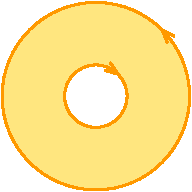
\includegraphics{images/HW12_1}}\end{picture}
    \vspace{-2pt}

  \end{enumerate}
%%%%%%%%%%%%%%%%%%%%%%%%%%%%%%%%%%%%%%%%%%%%%%%%%%%%%%%%%%%%%%%%%%%%%%%%%%%%%%%%%%%%%%%%%%%%%%%%%%%%
   
%%%%%%%%%%%%%%%%%%%%%%%%%%%%%%%%%%%%%%%%%%%%%%%%%%%%%%%%%%%%%%%%%%%%%%%%%%%%%%%%%%%%%%%%%%%%%%%%%%%%
\item Let $k>2$ be an integer.
  Find the area of the  region bounded by the {\color{blue}\sl $k$-hypocycloid} with  vector equation \newline
    $\bfr(t)= \bigl(a(k{-}1)\cos t+a\cos((k{-}1) t)\bigr)\bfi + \bigl(a(k{-}1)\sin t-a\sin((k{-}1) t)\bigr) \bfj$.
    
    \begin{picture}(382,95)(0,-10)
      \put( 10,0){\includegraphics{images/HW12_2}}      \put(  0,-10){$k=3$, deltoid}
      \put(100,0){\includegraphics{images/HW12_3}}  \put(100,-10){$k=4$, astroid}
      \put(200,0){\includegraphics{images/HW12_4}}      \put(200,-10){$k=5$, pentoid}
      \put(300,0){\includegraphics{images/HW12_5}}       \put(300,-10){$k=6$, hexoid?}
    \end{picture}
 \vspace{-2pt}
%%%%%%%%%%%%%%%%%%%%%%%%%%%%%%%%%%%%%%%%%%%%%%%%%%%%%%%%%%%%%%%%%%%%%%%%%%%%%%%%%%%%%%%%%%%%%%%%%%%%

   
%%%%%%%%%%%%%%%%%%%%%%%%%%%%%%%%%%%%%%%%%%%%%%%%%%%%%%%%%%%%%%%%%%%%%%%%%%%%%%%%%%%%%%%%%%%%%%%%%%%%
\item  Let $S$ be a region in the $xy$-plane with boundary $C$.
  Show that its moments $M_x$ and $M_y$ about the $x$- and $y$- axes are given by
  \[
  M_x\ =\ -\frac{1}{2}\oint_C y^2\, dx\quad \mbox{ and }\
  \quad
  M_y\ =\  \frac{1}{2}\oint_C x^2\, dy\,, \vspace{-2pt}
  \]
  where $S$ has constant mass density.
 \vspace{-2pt}
%%%%%%%%%%%%%%%%%%%%%%%%%%%%%%%%%%%%%%%%%%%%%%%%%%%%%%%%%%%%%%%%%%%%%%%%%%%%%%%%%%%%%%%%%%%%%%%%%%%%

   
%%%%%%%%%%%%%%%%%%%%%%%%%%%%%%%%%%%%%%%%%%%%%%%%%%%%%%%%%%%%%%%%%%%%%%%%%%%%%%%%%%%%%%%%%%%%%%%%%%%%
\item Use the previous problem to find the centroid of a semicircular region of radius $a$.
%%%%%%%%%%%%%%%%%%%%%%%%%%%%%%%%%%%%%%%%%%%%%%%%%%%%%%%%%%%%%%%%%%%%%%%%%%%%%%%%%%%%%%%%%%%%%%%%%%%%

  
  
%%%%%%%%%%%%%%%%%%%%%%%%%%%%%%%%%%%%%%%%%%%%%%%%%%%%%%%%%%%%%%%%%%%%%%%%%%%%%%%%%%%%%%%%%%%%%%%%%%%%
\item (Area of a polygon)
    Let $v_0=(x_0,y_0)$, $v_1=(x_1,y_1)$, \ldots, $v_n=(x_n,y_n)$ with $v_0=v_n$ be the vertices of a simple polygon $P$ in the plane,
    labeled counterclockwise.
    Show each of the following.
    %%%%%%%%%%%%%%%%%%%%%%%%%%%%%%%%%%%%%%%%%%%%%%%%%%
    \begin{enumerate}
    \item ${\displaystyle \int_C x\,dy\ =\ \frac{1}{2}}(x_1+x_0)(y_1-y_0)$, where $C$ is the edge $v_0 v_1$.

    \item The area of $P$ is ${\displaystyle \sum_{i=1}^n \frac{1}{2}(x_i+x_{i-1})(y_i-y_{i-1})  }$.

    \item The area of a polygon whose coordinates are integers (a {\color{blue}\sl lattice polygon}) is always a multiple of $\frac{1}{2}$.

    \item Check the formula for the polygon with vertices $(2,0)$, $(2,-2)$, $(6,-2)$, $(6,0)$, $(10,4)$, and $(-2,4)$.  \vspace{-2pt}
      
    \end{enumerate}
    %%%%%%%%%%%%%%%%%%%%%%%%%%%%%%%%%%%%%%%%%%%%%%%%%%
%%%%%%%%%%%%%%%%%%%%%%%%%%%%%%%%%%%%%%%%%%%%%%%%%%%%%%%%%%%%%%%%%%%%%%%%%%%%%%%%%%%%%%%%%%%%%%%%%%%%

     



    
\end{enumerate}



\end{document}
%%%%%%%%%%%%%%%%%%%%%%%%%%%%%%%%%%%%%%%%%%%%%%%%%%%%%%%%%%%%%%%%%%%
polar/Lune

   
%%%%%%%%%%%%%%%%%%%%%%%%%%%%%%%%%%%%%%%%%%%%%%%%%%%%%%%%%%%%%%%%%%%%%%%%%%%%%%%%%%%%%%%%%%%%%%%%%%%%
\item 
\vspace{-2pt}
%%%%%%%%%%%%%%%%%%%%%%%%%%%%%%%%%%%%%%%%%%%%%%%%%%%%%%%%%%%%%%%%%%%%%%%%%%%%%%%%%%%%%%%%%%%%%%%%%%%%
   
